\documentclass[10pt]{article}
\usepackage[left=1.5cm, right=1.5cm, top=0.8in, bottom=0.7in]{geometry}
\usepackage{fancyhdr}
\pagestyle{fancy}
\usepackage{lastpage}
\usepackage[most,breakable]{tcolorbox}
\usepackage{pdfcol,xcolor}
\usepackage{tikz}
\usepackage[linesnumbered,ruled,vlined]{algorithm2e}
%\usepackage{url}
\usepackage{dsfont}
\usepackage{amssymb,amsmath}
\usepackage{xspace}
\usepackage[normalem]{ulem}
\usepackage{bm}
\usepackage{enumitem}
\usepackage[breaklinks=true,colorlinks,linkcolor=magenta,urlcolor=magenta,citecolor=black]{hyperref}
\usepackage{cleveref}
\usepackage{xpatch}
\xpretocmd{\algorithm}{\hsize=\linewidth}{}{}

\newtcolorbox[auto counter]{exercise}[1][]{%
	colback=yellow!10,colframe=red!75!black,coltitle=white,use color stack,enforce breakable,enhanced,fonttitle=\bfseries,before upper={\parindent15pt\noindent}, title={\color{white}Exercise~\thetcbcounter: #1}}
\pagecolor{yellow!10}

\lhead{\textbf{University of Waterloo}}
\rhead{\textbf{2024 Spring}}
\chead{\textbf{CS480/680}}
\rfoot{\thepage/\pageref*{LastPage}}
\cfoot{\textbf{Yao-Liang Yu (yaoliang.yu@uwaterloo.ca) \textcopyright 2024}}

\newcommand{\pf}{\mathfrak{p}}
\newcommand{\qf}{\mathfrak{q}}
\newcommand{\pb}{\bar{p}}
\newcommand{\qb}{\bar{q}}
\newcommand{\pfb}{\bar{\mathfrak{p}}}
\newcommand{\qfb}{\bar{\mathfrak{q}}}
\newcommand{\rK}{\reflectbox{\ensuremath{K}}}
\newcommand{\lb}{\mathtt{lb}}
\newcommand{\ub}{\mathtt{ub}}
\newcommand{\mi}{\mathtt{maxiter}}
\newcommand{\tol}{\mathtt{tol}}
\newcommand{\softmax}{\mathsf{softmax}}
\newcommand{\KL}{\mathsf{KL}}

\newcommand{\bv}{\mathbf{b}}
\newcommand{\ev}{\mathbf{e}}
\newcommand{\fv}{\mathbf{f}}
\newcommand{\gv}{\mathbf{g}}
\newcommand{\pv}{\mathbf{p}}
\newcommand{\qv}{\mathbf{q}}
\newcommand{\rv}{\mathbf{r}}
\newcommand{\uv}{\mathbf{u}}
\newcommand{\wv}{\mathbf{w}}
\newcommand{\xv}{\mathbf{x}}
\newcommand{\yv}{\mathbf{y}}
\newcommand{\zv}{\mathbf{z}}
\newcommand{\gbs}{\bm{\mathsf{g}}}
\newcommand{\wbs}{\bm{\mathsf{w}}}
\newcommand{\xbs}{\bm{\mathsf{x}}}
\newcommand{\Xv}{\mathbf{X}}
\newcommand{\Yv}{\mathbf{Y}}
\newcommand{\Bsf}{\mathsf{B}}
\newcommand{\Lsf}{\mathsf{L}}
\newcommand{\Usf}{\mathsf{U}}
\newcommand{\Xsf}{\mathsf{X}}
\newcommand{\Ysf}{\mathsf{Y}}
\newcommand{\Zsf}{\mathsf{Z}}
\newcommand{\Dc}{\mathcal{D}}
\newcommand{\Nc}{\mathcal{N}}
\newcommand{\EE}{\mathds{E}}
\newcommand{\RR}{\mathds{R}}
\newcommand{\alphav}{\boldsymbol{\alpha}}
\newcommand{\betav}{\boldsymbol{\beta}}
\newcommand{\epsilonv}{\boldsymbol{\epsilon}}
\newcommand{\gammav}{\boldsymbol{\gamma}}

\newcommand{\ans}[1]{{\color{blue}\textsf{Ans}: #1}}
\newcommand{\argmin}{\mathop{\mathrm{argmin}}}
\newcommand{\argmax}{\mathop{\mathrm{argmax}}}
\newcommand{\diag}{\mathrm{diag}}
\newcommand{\dinner}[2]{\langle\!\langle#1,#2\rangle\!\rangle}
\newcommand{\inner}[2]{\langle #1, #2 \rangle}
\newcommand{\one}{\mathbf{1}}
\newcommand{\pred}[1]{[\![#1]\!]}
\newcommand{\prox}[1]{\mathrm{P}_{#1}}
\newcommand{\sgm}{\mathsf{sgm}}
\newcommand{\sign}{\mathop{\mathrm{sign}}}
\newcommand{\tr}{\mathrm{tr}}
\newcommand{\zero}{\mathbf{0}}

\newcommand{\ea}{{et al.}\xspace}
\newcommand{\eg}{{e.g.}\xspace}
\newcommand{\ie}{{i.e.}\xspace}
\newcommand{\iid}{{i.i.d.}\xspace}
\newcommand{\cf}{{cf.}\xspace}
\newcommand{\wrt}{{w.r.t.}\xspace}
\newcommand{\aka}{{a.k.a.}\xspace}
\newcommand{\etc}{{etc.}\xspace}

\newcommand{\red}[1]{{\color{red}#1}}
\newcommand{\blue}[1]{{\color{blue}#1}}
\newcommand{\magenta}[1]{{\color{magenta}#1}}
\newcommand{\green}[1]{{\color{green}#1}}
%===========================================================
\begin{document}

\begin{center}
	\large{\textbf{CS480/680: Introduction to Machine Learning} \\ Homework 3\\ \red{Due: 11:59 pm, July 08, 2024}, \red{submit on LEARN}.} \\

	{\bf \green{NAME}} \\
	{\bf \green{student number}}

\end{center}

\begin{center}
	Submit your writeup in pdf and all source code in a zip file (with proper documentation). Write a script for each programming exercise so that the TA can easily run and verify your results. Make sure your code runs!

	[Text in square brackets are hints that can be ignored.]
\end{center}

\begin{exercise}[Vision Transformers (10 pts)]
	Please follow the instructions of this \href{https://cs.uwaterloo.ca/~y328yu/mycourses/480/a3-vit.ipynb}{\texttt{ipynb} file}.

	\begin{enumerate}
		\item (1+3+2 = 6 pts) Complete the missing coding parts in the provided \href{https://cs.uwaterloo.ca/~y328yu/mycourses/480/a3-vit.ipynb}{\texttt{ipynb} file}.

		\item (1 pt) Visualization of patches:

		      
\includegraphics[width=.45\textwidth]{img/img_grid_0.png}
\includegraphics[width=.45\textwidth]{img/img_grid_1.png}

		      
\includegraphics[width=.45\textwidth]{img/img_grid_2.png}
\includegraphics[width=.45\textwidth]{img/img_grid_3.png}

		\item (1 pt) The test accuracy I obtained on MNIST is: 92.9\%

		\item (2 pts) Training / Validation accuracy  vs. epoch:

		      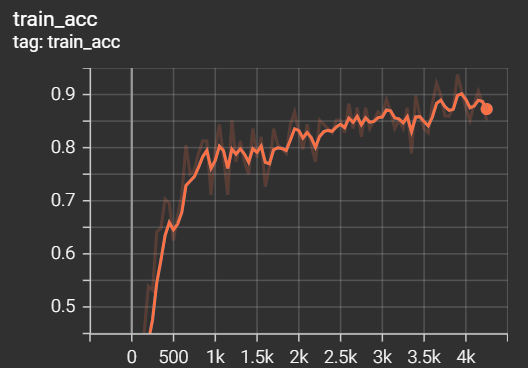
\includegraphics[width=.45\textwidth]{img/train_acc.png}
		      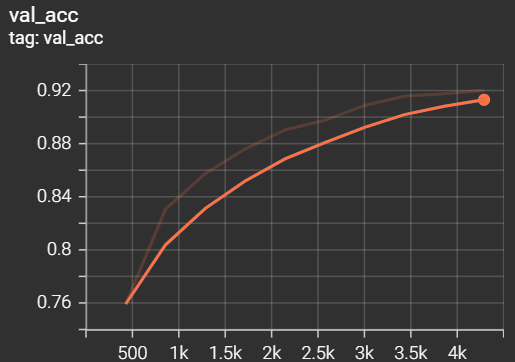
\includegraphics[width=.45\textwidth]{img/val_acc.png}
	\end{enumerate}
\end{exercise}

\newpage

\begin{exercise}[Adaboost (8 pts)]
	In this exercise we will implement Adaboost. Recall that Adaboost aims at minimizing the exponential loss:
	\begin{align}
		\min_{\wv} ~ \sum_i \exp \left( - y_i \sum_j  w_j h_j(\xv_i) \right),
	\end{align}
	where $h_j$ are the so-called weak learners, and the combined classifier
	\begin{align}
		\label{eq:combined-classifer}
		h_{\wv}(\xv) := \sum_j w_j h_j(\xv).
	\end{align}
	Note that we \red{assume $y_i \in \{\pm 1\}$} in this exercise, and we \red{simply take $h_j(\xv) = \sign(\pm x_j + b_j)$} for some $b_j \in \RR$.
	Upon \red{defining $M_{ij} = y_i h_j(\xv_i)$}, we may simplify our problem further as:
	\begin{align}
		\label{eq:adaboost-obj}
		\min_{\wv\in \RR^d} ~ \one^\top \exp(-M\wv),
	\end{align}
	where $\exp$ is applied component-wise and $\one$ is the vector of all 1s.

	Recall that $(s)_+ = \max\{s, 0\}$ is the positive part while $(s)_- = \max\{-s, 0\} = |s| - s_+$.

	\begin{algorithm}[H]
		\DontPrintSemicolon
		\KwIn{$M\in\RR^{n\times d}$, $\wv_0= \zero_d$, $\pv_0=\one_n$, $\mathsf{max\_pass} = 300$}

		\KwOut{$\wv$}

		\For{$t=0, 1, 2, \ldots, \mathsf{max\_pass}$ }{

			$\pv_t \gets \pv_t / (\one^\top \pv_t)$ \tcp*{normalize}

			$\epsilonv_t \gets (M)_-^\top \pv_t $ \tcp*{ $(\cdot)_-$ applied component-wise }

			$\gammav_t \gets  (M)_+^\top \pv_t $ \tcp*{$(\cdot)_+$ applied component-wise}

			$\betav_{t} \gets \frac12(\ln\gammav_{t} - \ln\epsilonv_t)$ \tcp*{$\ln$ applied component-wise}

			choose $\alphav_t \in \RR^d$  \tcp*{decided later}

			$\wv_{t+1} \gets \wv_t + \alphav_t \odot \betav_t$  \tcp*{$\odot$ component-wise multiplication}

			$\pv_{t+1} \gets \pv_t \odot \exp( - M (\alphav_t \odot \betav_t) ) $  \tcp*{$\exp$ applied component-wise}
		}
		\caption{Adaboost.}
		\label{alg:adaboost}
	\end{algorithm}

	\begin{enumerate}
		\item (2 pts) We claim that \Cref{alg:adaboost} is indeed the celebrated Adaboost algorithm if the following holds:
		      \begin{itemize}
			      \item $\alphav_t$ is one-hot (i.e., 1 at some entry and 0 everywhere else), namely, it indicates which weak classifier is chosen at iteration $t$.
			      \item $M \in \{\pm1\}^{n\times d}$, \ie, if all weak classifiers are $\{\pm 1\}$-valued.
		      \end{itemize}
		      With the above conditions, \uline{prove that (a)} $\gammav_t = \one - \epsilonv_t$, and \uline{(b) the equivalence} between \Cref{alg:adaboost} and the Adaboost algorithm in class. [Note that our labels here are $\{\pm1\}$ and our $\wv$ may have nothing to do with the one in class.]

		      \ans

		      \uline{Part (a): Prove that $\gammav_t = \one - \epsilonv_t$}

		      Since $M \in \{\pm1\}^{n \times d}$:
		      \begin{itemize}
			      \item $(M_{ij})_+ = \max(M_{ij}, 0)$, meaning $(M_{ij})_+ = 1$ if $M_{ij} = 1$ and 0 if $M_{ij} = -1$.
			      \item $(M_{ij})_- = \max(-M_{ij}, 0)$, meaning $(M_{ij})_- = 1$ if $M_{ij} = -1$ and 0 if $M_{ij} = 1$.
		      \end{itemize}

		      Therefore, for any entry $M_{ij}$, we have:
		      $$
			      (M_{ij})_+ + (M_{ij})_- = 1
		      $$

		      Then, for any fixed $j$, we have:
		      $$
			      \gammav_{tj} + \epsilonv_{tj} = \sum_i (M_{ij})_+ \pv_{ti} + \sum_i (M_{ij})_- \pv_{ti} = \sum_i \pv_{ti} = 1
		      $$

		      Thus:
		      $$
			      \gammav_t = \one - \epsilonv_t
		      $$

		      \uline{Part (b): Prove the Equivalence Between the Algorithm and Adaboost}

		      \textbf{Step 1}: Normalization

		      In the given AdaBoost algorithm from the exercise, we normalize $\pv_t$ directly:
		      $$ \pv_t \gets \pv_t / (\one^\top \pv_t) $$

		      In the class AdaBoost algorithm, we normalize the weights $\mathbf{w}_t$ to get $\mathbf{p}_t$:
		      $$ \mathbf{p}_t = \mathbf{w}_t / \langle \mathbf{1}, \mathbf{w}_t \rangle $$

		      Here, $\pv_t$ in the exercise algorithm corresponds to $\mathbf{p}_t$ and $\mathbf{w}_t$ in the class AdaBoost algorithm.

		      \textbf{Step 2}: Error Calculation

		      In the exercise algorithm, the weighted errors are calculated as:
		      $$ \epsilonv_t = (M)_-^\top \pv_t $$
		      $$ \gammav_t = (M)_+^\top \pv_t $$

		      Since we proved that $\gammav_t = \one - \epsilonv_t$, this matches the error calculation in the class AdaBoost algorithm, where the weighted error $\epsilon_t$ is:
		      $$ \epsilon_t = \sum_{i=1}^n p_{it} |h_t(x_i) - y_i| $$
		      $|h_t(x_i) - y_i|$ is litearlly the same as $(M)_-$ that is used to select the samples misclassified by weak learners.

		      \textbf{Step 3}: Beta Calculation

		      In the given algorithms, $\beta_t$ is calculated as:
		      $$ \betav_t = \frac{1}{2} \left( \ln(\gammav_t) - \ln(\epsilonv_t) \right)= \frac{1}{2} \ln \left( \frac{1 - \epsilon_t}{\epsilon_t} \right) $$

		      In the class AdaBoost algorithm:
		      $$ \beta_t = \frac{\epsilon_t}{1 - \epsilon_t} $$

		      They are not completely equivalent. However, in the given algorithm, $\betav_t$ will multiply by $\alphav_t$ which is used to select the error that are associated with the chosen weak learner and then accumulated in the output $\wv$:
		      $$ \wv_{t+1} \gets \wv_t + \alphav_t \odot \betav_t $$
		      And in the class algorithm, $\beta_t$ will be stored and expressed in the output meta-classifier as:

		      $$\ln\left(\frac{1}{\beta_t}\right) = \ln \left( \frac{1 - \epsilon_t}{\epsilon_t} \right)$$

		      Thus, $\betav_t$ and $\beta_t$ ultimately play the same role and $h_\wv(\xv)$ is equivalent to $\overline{h}$.
		      %   (the existence of $\frac{1}{2}$ is due to different labels in two algorithm: $\{\pm1\}$ vs. $\{0, 1\}$)

		      \textbf{Step 4}: Weight Update

		      In the exercise algorithm, weights are updated as:
		      $$ \pv_{t+1} \gets \pv_t \odot \exp(-M (\alphav_t \odot \betav_t)) $$

		      In the class AdaBoost algorithm:
		      $$ \mathbf{w}_{t+1} = \mathbf{w}_t \odot \beta_t^{\ell_t} $$

		      Since $\alphav_t$ is one-hot, $\exp(-M (\alphav_t \odot \betav_t))$ only computes the loss associated with the chosen weak learner and then update the weight according to the value of the computed loss, matching the concept in the class AdaBoost algorithm where weights are updated based on the weak classifier's performance.

		      \newpage

		\item (2 pts) Let us derive each weak learner $h_j$. Consider each feature in turn, we train $d$ linear classifiers that each aims to minimize the weighted training error:
		      \begin{align}
			      \min_{b_j\in \RR, s_j \in \{\pm1\}} ~ \sum_{i=1}^n ~ p_i \pred{ y_i (s_j x_{ij} + b_j) \leq 0  },
		      \end{align}
		      where the weights $p_i \geq 0$ and $\sum_i p_i = 1$.
		      \uline{Find (with justification)} an optimal value for each $b_j$ and $s_j$. [If multiple solutions exist, you can use the middle value.]
		      If it helps, you may assume $p_i$ is uniform, i.e., $p_i \equiv \tfrac1n$.

		      \ans

		      First, sort the unique $j$th features:
		      $$ x_{i_1j} \le x_{i_2j} \le \ldots \le x_{i_kj}.$$
		      Consider possible thresholds for $ b_j $ as the midpoints between each pair of adjacent sorted feature values. These midpoints are $ \tilde{x}_{a,j} = \frac{x_{i_aj} + x_{i_{a+1}j}}{2} $ for $ a = 1, 2, \ldots, k-1 $ and $\tilde{x}_{0,j}=x_{i_1j}-\epsilon, \tilde{x}_{k,j}=x_{i_kj}+\epsilon$ for edge cases. Each threshold is a fence to split the dataset into two classes and $ s_j \in \{\pm1\} $ is using to decide how to classify each class.

		      For each candidate threshold $ \tilde{x}_{k,j} $, calculate the weighted error for $ s_j = +1 $:
		      $$
			      \text{error}(+1; -\tilde{x}_{k,j}) = \sum_{i=1}^n p_i \pred{ y_i (x_{ij} - \tilde{x}_{k,j}) \leq 0 }.
		      $$
		      This means we are considering the classifier $ h_j(\xv_i) = \sign(x_{ij} - \tilde{x}_{k,j}) $.

		      For $ s_j = -1 $, we calculate the weighted error as:
		      $$
			      \text{error}(-1; \tilde{x}_{k,j}) = \sum_{i=1}^n p_i \pred{ y_i (-x_{ij} + \tilde{x}_{k,j}) \leq 0 }.
		      $$
		      This means we are considering the classifier $ h_j(\xv_i) = \sign(-x_{ij} + \tilde{x}_{k,j}) $.

		      Finally, find the optimal $ s_j $ and $ \tilde{x}_{k,j} $ that minimize the weighted error:
		      $$
			      \boxed{(s_j^*, b_j^*) = \arg\min_{s_j \in \{\pm1\}, b_j \in \left\{-s_j\tilde{x}_{a,j} \mid a = 0, \ldots, k\right\}} \sum_{i=1}^n p_i \pred{ y_i (s_j x_{ij} + b_j) \leq 0 }}.
		      $$

		\item (2 pts) [Parallel Adaboost.] \uline{Implement} \Cref{alg:adaboost} with the following choices:
		      \begin{itemize}
			      \item $\alphav_t \equiv \one$
			      \item pre-process $M$ by dividing a constant so that for all $i$ (row), $\sum_j |M_{ij}| \leq 1$.
		      \end{itemize}
		      \uline{Run} your implementation on the \href{https://archive.ics.uci.edu/dataset/350/default+of+credit+card+clients}{default} dataset (available on \href{https://cs.uwaterloo.ca/~y328yu/mycourses/480/assignment.html}{course website}), and \uline{report the training loss in \eqref{eq:adaboost-obj}, training error, and test error w.r.t. the iteration $t$,} where
		      \begin{align}
			      \label{eq:error}
			      \mathrm{error}(\wv; \Dc) := \frac{1}{|\Dc|}\sum_{ (\xv, y) \in \Dc} ~\pred{y h_{\wv}(\xv) \leq 0}.
		      \end{align}
		      [Recall that $h_\wv(\xv)$ is defined in \eqref{eq:combined-classifer} while each $h_j$ is decided in Ex~2.2. In case you fail to determine $h_j$, in Ex~2.3 and Ex~2.4 you may simply use $h_j(\xv) = \sign(x_j-m_j)$ where $m_j$ is the median value of the $j$-th feature in the training set.]

		      [Note that $\wv_t$ is dense (i.e., using all weak classifiers) even after a single iteration.]

		      \ans{
			      We report all 3 curves in one figure, with clear coloring and legend to indicate which curve is which.
			      \begin{center}
				      \includegraphics[width=.5\textwidth]{plot/ex2q3.png}
			      \end{center}
		      }

		\item (2 pts) [Sequential Adaboost.]  \uline{Implement} \Cref{alg:adaboost} with the following choice:
		      \begin{itemize}
			      \item $j_t = \argmax_j | \sqrt{\epsilon_{t,j}} - \sqrt{\gamma_{t,j}} |$ and $\alphav_t$ has 1 on the $j_t$-th entry and 0 everywhere else.
			      \item pre-process $M$ by dividing a constant so that for all $i$ and $j$, $|M_{ij}| \leq 1$.
		      \end{itemize}
		      \uline{Run} your implementation on the \href{https://archive.ics.uci.edu/dataset/350/default+of+credit+card+clients}{default} dataset (available on \href{https://cs.uwaterloo.ca/~y328yu/mycourses/480/assignment.html}{course website}), and \uline{report the training loss in \eqref{eq:adaboost-obj}, training error, and test error in \eqref{eq:error} w.r.t. the iteration $t$.}

		      [Note that $\wv_t$ has at most $t$ nonzeros (i.e., weak classifiers) after $t$ iterations.]

		      \ans{
			      We report all 3 curves in one figure, with clear coloring and legend to indicate which curve is which.
			      \begin{center}
				      \includegraphics[width=.5\textwidth]{plot/ex2q4.png}
			      \end{center}
		      }

	\end{enumerate}
\end{exercise}

\end{document}
